  %% da_manual_DE.tex
  %% Copyright 2015 Simon M. Laube
  %
  % This work may be distributed and/or modified under the
  % conditions of the LaTeX Project Public License, either version 1.3
  % of this license or (at your option) any later version.
  % The latest version of this license is in
  %   http://www.latex-project.org/lppl.txt
  % and version 1.3 or later is part of all distributions of LaTeX
  % version 2005/12/01 or later.
  %
  % This work has the LPPL maintenance status `author maintained'.
  % 
  % The Current Maintainer of this work is S. M. Laube
  %
  % This work consists of the files listed in ./Help/files.txt
  
%%~~~~~~~~~~~~~~~~~~~~~~~~~~~~~~~~~~~~~~~~~~~%% 
%%    Documentation of the etdipa-template   %%
%%~~~~~~~~~~~~~~~~~~~~~~~~~~~~~~~~~~~~~~~~~~~%%
\PassOptionsToPackage{xcolor}{dvipsnames}
\documentclass[12pt,paper=a4]{scrartcl}
\usepackage[utf8]{inputenc}
\usepackage[naustrian]{babel}
\usepackage[scale=0.7]{geometry}
\usepackage{graphicx}
\usepackage{float}
\usepackage{circuitikz}
\usepackage{listings}
\usepackage{array}




\lstset{language=[LaTeX]TeX,
		texcsstyle=*\ttfamily\color{red!80!black},
		literate={{ß}{{\ss}}2},
		basicstyle={\ttfamily\color{black}},
		commentstyle=\color{green!60!black},
		keywordstyle=\ttfamily\color{red!80!black},
		numberstyle=\tiny\color{red},
		numbers=left,
		captionpos=b,
		%otherkeywords={},
		basicstyle=\footnotesize,		
		morekeywords={\diplomand ,\breite ,\@width@dpl ,\@sep@dpl,\ifundefined,
					  \@breite,\@default@breite,\setlength,\providecommand,{\ },{\\},\includegraphics,
					  \responsible,\hypersetup,\tikz,\",\href,\node,\dipalistoffigures,$, \{, \}, \[, \],\includepdf,\frontmatter,\appendix,\mainmatter,\schuljahr,\professor,\maketitle,\addchap,\acro,\unterschrift,\usetikzlibrary,\includepdf, \schule,\firma, \Masse,\TikZ,\S,\D,\DS,\SD,\dipacolor,\@@eid@text,\definecolor
\dipalistoffigures,\dipalistoftables,\dplversion,\ETdipaversion,\manversion,\dokumenttyp,\dipvorname,\eidname,\dankname,
\definecolor,\place,\setmyheadings}
		}
		
		\usepackage{etdipa}
		\clearscrheadfoot\relax
		\pagestyle{empty}
		\pagestyle{scrheadings}
		

\setfootsepline{.5pt}
\setheadsepline{.5pt}
\ohead{\today}
\ihead{Simon~Michael~Laube}
\ifoot{{\ttfamily etdipa} -- Manual}
\ofoot{\pagemark}


\title{Verwendung des Diplomarbeits-Templates \ETdipaversion}
\author{Simon~Michael~Laube\\5BHET~2014/15}
\date{\today}
\def\TikZ{Ti\textit{k}Z}
\def\addtoc#1#2{\addcontentsline{toc}{#1}{#2}}
\def\nsec#1{\section*{#1}\addtoc{section}{#1}}
\def\nsubsec#1{\subsection*{#1}\addtoc{subsection}{#1}}
\def\nsubsubsec#1{\subsubsection*{#1}\addtoc{subsubsection}{#1}}
\setlength{\parindent}{0pt}

%% DIRTY TRICK :)
\makeatletter
\def\maketitle{%
\thispagestyle{empty}
\begin{figure}[H]
\includegraphics[scale=1]{Images/ET_logo.jpg}
\centering
\end{figure}
\begin{center}
	\Huge \bfseries\sffamily\@title\\
	\vskip 1em
	\Large\mdseries\rmfamily\@author\\
	\vskip .5em
	\large\mdseries\@date\\
	\normalsize	\rmfamily
\end{center}
				}%
\makeatother

\usepackage[colorlinks=true,
			linkcolor=black,
			citecolor=green,
			urlcolor=blue,
			bookmarks=true,
			bookmarksopen=true]{hyperref}

\begin{document}

\maketitle
\tableofcontents\newpage


\addtocontents{toc}{\protect \large {\bfseries Teil~I: Konventionen \& Struktur}\protect\vspace{1mm}\hrule\normalsize}

\nsec{Vorwort}\vspace{-1mm}
Dieses Template mit den beiliegenden Dateien dient der Erstellung
einer Diplom\-arbeits\-dokumentation, oder einem ähnlich anspruchsvollen
Dokument\footnote{Bitte beachten Sie, dass das Template
für die {\ttfamily scrreprt} Klasse geschrieben wurde.}, mit dem \TeX{} Makropaket \LaTeX{}.
Der Aufbau des Templates ist dabei so einfach wie möglich um jede
Könnerstufe von \LaTeX{}-Benutzern dazu anzuregen, ihre Diplomarbeit
mit \LaTeX{} zu verfassen. Gewisse Befehle
gehören jedoch zum Mindestmaß an Syntax und werden daher ohne
jede Erklärung verwendet.\par\medskip

Diese Vorlage soll eine Richtlinie und Hilfe für die Erstellung
der Diplomarbeitsdokumentation sein. Sie ersetzt nicht die
Gestaltung von typografisch und sprachlich richtigen Texten und Strukturen.
\par\medskip

Seit der vorliegenden Version \ETdipaversion{} ist das Template so 
modifizierbar, dass es auch für Vor\-wiss\-en\-schaft\-liche Arbeiten (VWA)
verwendbar ist. Für weiterführende Informationen 
lesen Sie bitte die \href{http://www.ctan.org/pkg/etdipa}{README} am CTAN-Server oder die 
komplette \href{https://medium.com/@simon_m_laube/etdipa-offical-release-details-by-the-author-59b6d9ad104b}{Projekthistorie}.\par \medskip
	
	
	Weiters sind Verbesserungsvorschläge oder Anregungen durchaus erwünscht. Sie können mich über
\href{mailto:simon.laube@gmx.at}{simon.laube@gmx.at} erreichen. Für Erklärungen zum
Template steht diese Adresse jedoch nicht zur Verfügung, dafür ist die vorliegende
Dokumentation gedacht. \par\vspace{-2mm}

\nsubsec{Danksagungen}
Ich möchte mich hiermit bei allen Personen bedanken, die zur Verbesserung des Templates beigetragen haben.
Ein besonderer Dank geht an Prof. Mag Dipl.-Ing. Dr.~Daniel~Asch und Prof. Dipl.-Ing. Dr. Wilhelm Haager
für die Betreuung des Projektes und der Unterstützung bei \TeX nischen Fragen.\par\medskip



\null\hfill -- Simon Michael Laube, \today{} -- 

\section{Konventionen}
In diesem Abschnitt sollen kurz die festgelegten Darstellungskonventionen
für \\dieses Dokument erläutert werden. \par\medskip
\begin{tabular}{>{\bfseries}c l}
Befehle &  werden im Folgenden immer in {\ttfamily Typewriter}-Schriftart,\\
		&  sowie in einer \textit{Listings-} oder 
			\textit{Verbatim}umgebung dargestellt. \\
&\\
Begriffe&  aus der \LaTeX{}-Welt und Hervorhebungen werden \textit{kursiv} gesetzt.
\end{tabular}\par\bigskip

Eine Übersicht über alle Templatebefehle befindet sich in Anhang~\ref{sec:befehle}.\par




\section{Strukturierung}

%% ==== Ordner ==== %%
\subsection{Ordnerstruktur}
\begin{figure}[H]
\centering
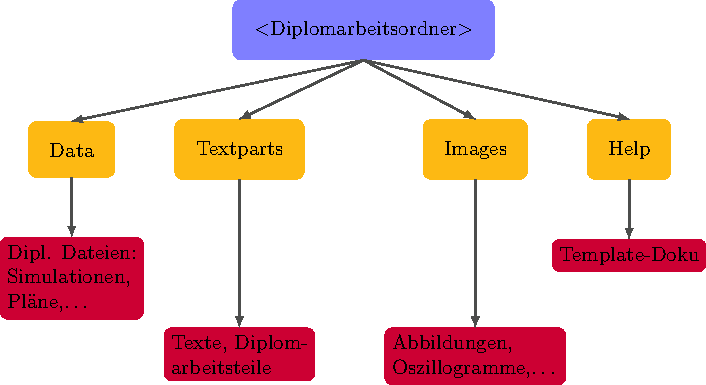
\includegraphics[width=0.7\textwidth]{Images/Ordnerstruktur.pdf}
\caption{Vorgegebene Ordnerstruktur im Diplomarbeitsordner\newline
		\protect\tikz{\protect\node[rectangle,fill=blue!50!white]{};} \dots\dots Stammordner\newline
		\protect\tikz{\protect\node[rectangle,fill=yellow!70!red]{};} \dots\dots Unterverzeichnisse\newline
		\protect\tikz{\protect\node[rectangle,fill=red!80!blue]{};} \dots\dots Erklärung}
\label{pic:ordnerstruktur}
\end{figure}

Abbildung~\ref{pic:ordnerstruktur} zeigt die festgelegte Ordnerstruktur im Diplomarbeitsordner. Für
den Benutzer sind im Wesentlichen nur die Ordner \textit{Data, Images} und \textit{Textparts} von Bedeutung.
Im \textit{Help} Ordner befindet sich die Dokumentation zum Diplomarbeitstemplate, also diese Datei.\par\bigskip

Die vorgegebene Struktur soll nicht verändert werden um eine gewisse Einheitlichkeit der Diplomarbeitsordner
für betreuende Lehrer und die eventuelle spätere Verwendung zu schaffen. Es dürfen -- und sollen -- 
Unterordner angelegt werden um die Übersicht zu verbessern. Ein Beispiel für solch eine Unterteilung ist in
Abbildung~\ref{pic:unterordner} zu sehen. Mehr zum Thema "`{Arbeiten mit
mehreren \LaTeX{}-Dateien}"' kann in Abschnitt~\ref{sec:master} nachgelesen werden.\par\vspace{1mm}
\begin{figure}[H]
\centering
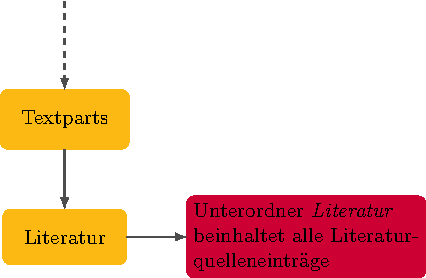
\includegraphics[width=0.4\textwidth]{Images/subordner.pdf}
\caption{Beispielhafte Unterteilung der vorgegebenen Ordner in Abbildung~\ref{pic:ordnerstruktur}}
\label{pic:unterordner}
\end{figure}

\def\labelitemi{$>$}
\begin{itemize}


\item Der \textit{Data} Ordner ist der Hauptordner der Diplomarbeit außerhalb der Dokumentation.
Er ist gedacht für Simulationdateien (z.B.: Proteus, {\scshape Spice}), technische Zeichnungen und
Diagramme (z.B.: AutoCAD, \TikZ), Stromlaufpläne (EPlan,\dots) und dergleichen. Bei Bedarf kann
auch die Diplomarbeitspräsentation (PowerPoint, Beamer-\LaTeX{}, Prezi) in diesem Ordner
abgelegt werden.

\item Der \textit{Textparts} Ordner ist das zentrale Element der Dokumentation. In ihm werden sämtliche
Subfiles der Doku abgelegt und verwaltet. In Abschnitt~\ref{sec:master} wird das Arbeiten mit
mehreren Dateien erläutert. In diesem Ordner werden auch sämtliche Hilfsdateien abgelegt, welche
in \LaTeX{} eingebunden werden (PDFs, eventuell externe Literaturverzeichnisse,\dots).

\item Der \textit{Images} Ordner dient dem/den Benutzer(n) als Ablage für alle Fotos und Bilder.
Zum einen sind das Fotos, welche in die Dokumentation eingebunden werden; zum anderen alle sonstigen Fotos
(Testversuche, usw.).

\end{itemize}\bigskip

Das Masterfile der Dokumentation liegt im Stammordner (vgl. Abbildung~\ref{pic:ordnerstruktur}) 
der Diplomarbeit und greift von dort aus auf die benötigten Daten in Unterordnern zu.\par\newpage

%% ==== Mastefile ==== %%
\subsection{Arbeiten mit Masterfile}\label{sec:master}
Im Folgenden wird das Arbeiten mit mehreren \LaTeX{}-Dateien erläutert. Für die
meisten Benutzer dieses Templates wird die erklärte Arbeitsweise neu sein; das Prinzip
ist unter \LaTeX{} Benutzern jedoch weit verbreitet.\par\bigskip

Im Grunde kann man zwischen zwei Fällen unterscheiden:
\begin{itemize}
\item[$-$] Das \LaTeX{}-File\footnote{Gilt für \LaTeXe{}. Da es sich um \TeX{}-Befehle handelt\\ aber analog in anderen Versionen
verwendbar.} hat eine angenehme Größe um die Übersicht nicht zu \\verlieren.
\item[$-$] Die Datei ist sehr groß und man verliert leicht die Übersicht über einzelne Dokumentteile.
\end{itemize}

Bei dem Ausmaß einer Diplomarbeitsdokumentation ist ohne Zweifel der zweite Fall gegeben.
Das dargestellte Problem lässt sich durch eine Umstellung der Arbeitsweise
mit \LaTeX{} vereinfachen. Nachfolgend dienen sogenannte \textit{Minimal\-beispiele} als 
Vorzeigeobjekte um Strukturen zu erklären.\par\bigskip

\subsubsection{Einzeldokument}
Bei kleineren Dokumenten arbeitet man mit einem \LaTeX{}-File, welches beispielsweise
so aussieht, wie in Listing~\ref{lst:normalesarbeiten} dargestellt.

\lstset{caption=Ein normales \LaTeX{} Dokument,label=lst:normalesarbeiten}
\begin{lstlisting}[ xleftmargin=.14\textwidth, xrightmargin=.14\textwidth]
%Dokumentklasse
\documentclass{article}
%UTF8 Encoding
\usepackage[utf8]{inputenc}
\begin{document}
	\section{Titel}
		Hier steht ein Text.
		\par %Absatzende
\end{document}
\end{lstlisting}

Beginnt die Dateigröße zu wachsen und wird die Übersicht trotz der Hilfe professioneller
Editoren immer schlechter, so kommt ein neues (und in \LaTeX{} durchaus übliches) System
zum Einsatz.\par \bigskip\bigskip

\subsubsection{Master- und Subfile}
Für sehr große Dokumente wird im ersten Schritt ein \textit{Masterfile} angelegt.
Meist enthält dieses die sogenannte Präambel (Usepackages usw.).\par Danach folgt
der Dokumentbeginn mit \verb|\begin{document}| und das Dokumentende mit 
\verb|\end{document}|. Listing~\ref{lst:masterfile} zeigt eine Möglichkeit
eines Masterfiles.\par

\lstset{caption=Ein \LaTeX{} Masterfile,label=lst:masterfile}
\begin{lstlisting}[ xleftmargin=.1\textwidth, xrightmargin=.1\textwidth]
%Praeambel
\documentclass{article}
\usepackage[utf8]{inputenc}
%Dokument Beginn
\begin{document}
	%vorerst noch leer
\end{document}
%Dokument Ende
\end{lstlisting}

Im zweiten Schritt erfolgt das Erstellen eines Textteils des Dokumentes 
in einer zweiten Datei (zum Beispiel \verb|meintext.tex|). Diese Datei 
enthält \textit{nur Text} und keine Präambel (siehe Listing~\ref{lst:subfile}).
Aus diesem Grund kann sie auch nicht als eigenständige Datei kompiliert, 
sondern nur gespeichert werden!\par
\lstset{caption=Ein \LaTeX{} Subfile,label=lst:subfile}
\begin{lstlisting}[ xleftmargin=.1\textwidth, xrightmargin=.1\textwidth]
%% file: meintext.tex
\section{Mein Textteil}
	Das ist ein Teil meines
	riesigen Dokumentes.\par
\end{lstlisting}\par\vspace{20mm}

Um das Hauptdokument mit Leben zu erfüllen wird der \TeX{} Befehl \verb|\input|
verwendet. Dafür muss der relative Dateipfad zur Masterdatei angegeben werden.
Für PDF-Dokumente kann der Befehl
\verb|\includepdf[<options>]{<name>}| verwendet werden. Dazu ist das Package {\ttfamily pdfpages} notwendig.
Im Allgemeinen soll das Einbinden von Dokumentteilen (ausgenommen Datenblätter oder ähnliches) als PDF
jedoch vermieden werden, da für Kopf- und Fußzeilen sonst zusätzliche Einstellungen notwendig werden.
Weiters kann eine PDF Datei nicht in voller Größe eingebunden werden, da Rücksicht auf die Seitenränder
genommen werden muss.\par

\lstset{caption=\LaTeX{} Masterfile mit eingebundenen Subfiles,label=lst:fullmaster}
\begin{lstlisting}[ xleftmargin=.1\textwidth, xrightmargin=.1\textwidth]
%Praeamble
\documentclass{article}
\usepackage[utf8]{inputenc}
\usepackage{pdfpages}
%Dokument Beginn
\begin{document}
	% Mein erster Teil %
	\input{meintext.tex}
	% Mein zweiter Teil% PDFs eher nicht
	\includepdf[pages=3-5]{meinepdf.pdf}
\end{document}
%Dokument Ende
\end{lstlisting}

\addtocontents{toc}{\protect\large\protect\newpage{\bfseries Teil~II: Verwendung des Templates}
\protect \vspace{1mm}\hrule\normalsize}

\section{Verwendung der Makros}\label{sec:macros}
In diesem Abschnitt werden die Funktionen des Templatepackages vorgestellt.
Die enthaltenen Makros wurden selbst definiert und gehören nicht zum
\LaTeX{}-Standard. Wichtig
dabei ist, dass der Benutzer nur das \verb|etdipa.sty| Package
einbinden muss. \par

\subsection{Titelseite -- {\ttfamily maketitle}}
Der \LaTeX{} Standardbefehl \verb|\maketitle| dient zur Erzeugung
von Titelseiten. Für die Verwendung in der Diplomarbeit wurde 
der Befehl umdefiniert und kann daher normal benutzt werden.
Wie in Standard \LaTeX{} müssen zur Erzeugung der Titelseite
die notwendigen Informationen vom Benutzer in der Präambel\footnote{oder
später, aber jedenfalls vor der Verwendung des maketitle-Befehls} 
angegeben werden.
Listing~\ref{lst:maketitle_info} zeigt die benötigten Angaben:

\lstset{caption=Informationen für die Titelseite,label=lst:maketitle_info}
\begin{lstlisting}[xleftmargin=.14\textwidth, xrightmargin=.14\textwidth]
%%==== Definitionen fuer die Diplomarbeit ====%%
\dokumenttyp{DIPLOMARBEIT}
\title{<Titel der Diplomarbeit>}
\author{Schueler 1 \and Schueler 2}
\place{<Ort>}
\date{<Datum>}
\schuljahr{<Schuljahr>}
\professor{Professor 1 \and Professor 2}
\dipacolor{ETred}
%%============================================%%
\end{lstlisting}

Zu Beginn der Diplomarbeit wird die Titelseite erzeugt
und daraufhin gleich die Verfasser gesetzt.\par\newpage
\lstset{caption=Beispielhafter Beginn der Diplomarbeit,label=lst:maketitle}
\begin{lstlisting}[xleftmargin=.15\textwidth, xrightmargin=.15\textwidth]
\begin{document}
\frontmatter
%%============ Titelseite ============%%
\maketitle
% Verantwortliche/Verfasser
\responsible{Schueler 1, Schueler 2}
%%====================================%%
             .     .     .
             .     .     .
             .     .     .
\end{lstlisting}


\subsection{Eidesstattliche Erklärung}
Die Eidesstattliche Erklärung wird über eine Umgebung hinzugefügt (siehe Listing~\ref{lst:eid}).
In dieser Umgebung müssen die Unterschriftenlinien für jeden Diplomanden gesetzt werden.
Die Eidesstattliche Erklärung benötigt eine ganze Seite und teilt sich die vertikalen Abstände
je nach Anzahl der Unterschriften selbst ein.\par 
\lstset{caption=Hinzufügen der Eidesstattlichen Erklärung,label=lst:eid}
\begin{lstlisting}[xleftmargin=.15\textwidth, xrightmargin=.15\textwidth]
%%===== Eidesstattliche Erklaerung ======%%
\begin{Eid}
%Unterschrift der Diplomanden hinzufuegen!
\unterschrift{Schueler 1}
\unterschrift{Schueler 2}
\end{Eid}\newpage
%%=======================================%%
\end{lstlisting}


\subsection{Danksagungen}
Der Text der Danksagungen wird in einer externen Datei verfasst 
und dann im Masterfile eingebunden (vgl. Abschnitt~\ref{sec:master}). 
Der Text selbst wird in einer Umgebung geschrieben:\par 
\lstset{caption=Hinzufügen der Danksagungen,label=lst:dank}
\begin{lstlisting}[xleftmargin=.15\textwidth, xrightmargin=.15\textwidth]
%% Danksagungen:
\begin{Danksagung}

%Wir bedanken uns bei \dots

\end{Danksagung}
\end{lstlisting}

\subsection{Literaturverzeichnis}
Literaturverzeichnisse zählen zu den wichtigsten Teilen eines technischen Dokumentes und sollen einheitlich gestaltet werden.
In \LaTeX{} gibt es die Möglichkeit externer Literaturdateien. Diese Methode erfordert jedoch ein großes Verständnis der 
Prozesse und ist daher nicht gut für schnelles Arbeiten geeignet.\par 

\LaTeX{} bietet eine Umgebung für Literaturverzeichnisse an. Für das Template wurde diese Umgebung leicht
angepasst und trägt daher auch einen anderen Namen. Die Verwendung erfolgt jedoch analog.
Ein Beispiel für einen Literatureintrag ist in Listing~\ref{lst:literatur} zu sehen.\par 

\lstset{caption=Literaturverzeichnis,label=lst:literatur}
\begin{lstlisting}[xleftmargin=.15\textwidth, xrightmargin=.15\textwidth]
%% Literaturverzeichnis:
\begin{Literatur}

\bibitem[1] % Nummer optional
        {TeXbook}% cite-key
        % TEXT:
        {\textbf{Donald~E.~Knuth:} 
        \emph{The \TeX{}book}. 
        1986, {\scshape Addison--Wesley} Verlag,
        ISBN-13: 978-0-201-13447-6}
        
\end{Literatur}
\end{lstlisting}
Der Literatureintrag in Listing~\ref{lst:literatur} ergibt Eintrag~\cite{TeXbook}.
Mit Hilfe des \verb|\cite| Makros kann im Text auf Quellen verwiesen werden. 
Alle Stellen aus anderen Quellen müssen im Text kenntlich gemacht werden!

\lstset{caption=Zitieren der Literaturquellen,label=lst:zitate}
\begin{lstlisting}[xleftmargin=.15\textwidth, xrightmargin=.15\textwidth]
%Zitieren im Text
Text~\cite{<cite-key>}
%z.B.:
Text~\cite{TeXbook}
\end{lstlisting}

\subsection{Abkürzungsverzeichnis}
Das Abkürzungsverzeichnis wird über das \textit{acronym}-Package von Tobias~Oetiker~\cite{acronym} gelöst.
Für die Diplomarbeit ist das Abkürzungsverzeichnis nur optional, da es nicht verwendet werden muss.
Listing~\ref{lst:abkuerz} zeigt ein Beispiel für das Erstellen eines Eintrags. Die Umgebung
funktioniert ähnlich dem Literaturverzeichnis. \par 
\newpage
\lstset{caption=Abkürzungsverzeichnis,label=lst:abkuerz}
\begin{lstlisting}[xleftmargin=.1\textwidth, xrightmargin=.1\textwidth]
% Abkuerzungsverzeichnis
%Kapitel ins Inhaltsverzeichnis einfuegen
\addchap{Abkuerzungsverzeichnis}
%Beginn  .....  Einrueckung (optional)
\begin{acronym}[ACRONYM]
%ein Eintrag:
%{Abkz. einfach}[Abkz. komplett]{Komplettes Wort}
\acro{ugs}[ugs.]{umgangssprachlich}                                                                                                                                                                                                                                                                                                                                                                                                                                                                                                                                                                                                                                                                                                                                                                                                                                                                                                                                                                                                                                                                                                                                                                                                                                                                                                                                                                                                                                                                                                                                                               
%Ende
\end{acronym}\newpage
\end{lstlisting}

Da dieses Verzeichnis nur optional ist wurde keine Anpassung 
wie beim Literaturverzeichnis vorgenommen.
Das Abkürzungsverzeichnis wird jedoch über \verb|\addchap| zum
Inhaltsverzeichnis hinzugefügt. Mittels \verb|\ac{<Abkz. einfach>}| kann
die Ab\-kürzung im Text verwendet werden.\par 


\subsection{Diplomandenvorstellung}\label{subsec:diplomand}
\begin{figure}[H]
\centering
\diplomand{Max~Mustermann}
		  {12.12.2012 in St.P\"olten}
		  {Langestra\ss e 13}
		  {3100 St.Pölten}
		  {\schule{2010--2015}{HTBLuVA St.Pölten, Abteilung für Elektrotechnik}
		  \schule{2006--2010}{Gymnasium XY}}
		  {max.muster@xy.at}
		  {Images/bild}
\caption{Ergebnis des Diplomandenvorstellungs-Makros}
\label{pic:diplomandenvorstellung}
\end{figure}\newpage

In der Diplomandenvorstellung werden die, im Projekt involvierten Schüler,
 nacheinander
vorgestellt. Die Vorstellung enthält einen kurzen Lebenslauf
der von den Schülern auszufüllen ist. Die Optik wurde
der \LaTeX{} Dokumentklasse {\ttfamily moderncv}\footnote{Dient
zur Erstellung hochwertiger Lebensläufe in verschiedenen
Farben und Designs.} nachempfunden und über \TikZ{} realisiert.\par 


\lstset{caption=Diplomandeneintrag erzeugen,label=lst:diplomandeneintrag}
\begin{lstlisting}[ xleftmargin=.15\textwidth, xrightmargin=.15\textwidth]
\begin{Diplomandenvorstellung}
   % Neuen Diplomandeneintrag erzeugen
   \diplomand
   {<Name>}
   {<Geburtsdaten>}
   {<Strasse>}
   {<PLZ Ort>}
   {<Schulen und Anstellungen>} 
   {<Email>}
   {<Dateiname_Bild>}
\end{Diplomandenvorstellung}
\end{lstlisting}
Listing~\ref{lst:diplomandeneintrag} zeigt den {\verb|\diplomand|}-Befehl.
Dieses Makro erzeugt mit den eingegebenen Daten (Makro-Argumente in $<\,>$)
eine Diplomandenvorstellung \textit{eines} Diplomanden 
(vgl. Abbildung~\ref{pic:diplomandenvorstellung}) und setzt dabei automatisch über \verb|\responsible| seinen Namen
als Verfasser in die Fußzeile.\par Die Argumente sind in der folgenden
Tabelle~\ref{tab:diplomand_arg} erklärt.\par
\medskip
Die Diplomandenvorstellungen müssen in der passenden Umgebung eingebunden werden.
Diese Umgebung setzt die Überschrift und stellt die Ausrichtung ein.
Einzelne Diplomandenvorstellungen können durch \verb|\newpage| getrennt werden.\par 
\begin{table}[H]
\centering
\begin{tabular}{l l}
\textbf{Argument}	& \textbf{Bedeutung}\\
\hline
$<$Name$>$			& Vor- und Familienname\\
$<$Geburtsdaten$>$	& Geburtsdaten in der Form \\
					& $<${\scshape Datum} in {\scshape Ort}$>$\\
$<$Straße$>$		& Straße und Hausnummer \\
$<$PLZ Ort$>$		& Postleitzahl und Wohnort\\
$<$Schulen und Anstellungen$>$& Schulen und Firmen\\
$<$Email$>$			& Email-Adresse\\
$<$Dateiname\underline{\ }Bild$>$& Dateipfad und Name des Bildes
\end{tabular}
\caption{Argumente des \textbackslash{\ttfamily diplomand}-Befehls}
\label{tab:diplomand_arg}
\end{table}\newpage


Die Breite des Schülerbildes kann dynamisch über den \verb|\breite|-Befehl
verändert werden. Es wird empfohlen den Wert nicht zu verändern, da
der Standardwert von $3\,\mathrm{cm}$ optimal erscheint.\par 

\lstset{caption=Breite des Diplomandenbildes einstellen,label=lst:breite}
\begin{lstlisting}[ xleftmargin=.2\textwidth, xrightmargin=.2\textwidth]
\breite{<Wert>}
\end{lstlisting}

\subsubsection{Einfügen der Schulen und Firmen}
Um in der Diplomandenvorstellung die Schulen und Firmen 
im beruflichen Werdegang einzufügen gibt es seit Version v2.4 die 
zwei Makros:
\lstset{caption=Firmen und Schulen einfügen,label=lst:firma_schule}
\begin{lstlisting}[ xleftmargin=.2\textwidth, xrightmargin=.2\textwidth]
\firma{<Zeitraum>}{<Firmenname>}
\schule{<Zeitraum>}{<Schulname>}
\end{lstlisting}
Die Befehle fügen lediglich die gewünschte Stelle im Werdegang
ein; die chronologische Ordnung muss vom Benutzer selbst vorgenommen werden.
Das folgende Listing~\ref{lst:diplomandenvorstellung} zeigt den 
Sourcecode zu Abbildung~\ref{pic:diplomandenvorstellung}.\par 

\lstset{caption=Beispiel einer Diplomandenvorstellung,label=lst:diplomandenvorstellung}
\begin{lstlisting}[ xleftmargin=.15\textwidth, xrightmargin=.15\textwidth]
\begin{Diplomandenvorstellung}
  \diplomand{Max~Mustermann}
  {12.12.2012 in St.P\"olten}
  {Langestra\ss e 13}
  {3100 St.P\"olten}
  {\schule{2010--2015}{HTBLuVA St.P\"olten, 
  Abteilung f\"ur Elektrotechnik}
  \schule{2006--2010}{Gymnasium XY}}
  {max.muster@xy.at}
  {Images/bild}
\end{Diplomandenvorstellung}
\end{lstlisting}

\subsection{Kopf- und Fußzeilen}
Die Kopf- und Fußzeilen sind über das \verb|scrpage2.sty| Package realisiert.
Die vorgegebene Formatierung wird im \verb|etdipa|-Package festgelegt und 
soll nicht verändert werden.
Zur Veränderung der Namen in der Fußzeile gibt es das \verb|\responsible| Makro
(vgl. Listing~\ref{lst:responsible}). Die Umstellung gilt ab der Seite auf
der diese vorgenommen wird. Bei zwei Definitionen auf einer Seite gilt
daher nur die letzte für die Fußzeile.\par\medskip

Sollten die Kopf- und Fußzeilen nicht im Dokument erscheinen, wurde 
vermutlich weder \verb|\frontmatter|, noch \verb|\mainmatter| verwendet.
Das Templatesetup kann in diesem Fall auch über \verb|\setmyheadings| am Beginn
des Dokuments eingestellt werden.\par\medskip

Jede Stelle im Text muss eindeutig einem Schüler zuzuordnen sein. Dazu wird
\verb|\responsible| verwendet.\par 

\lstset{caption=Namen in der Fußzeile ändern,label=lst:responsible}
\begin{lstlisting}[ xleftmargin=.2\textwidth, xrightmargin=.2\textwidth]
\responsible{<Name1>, <Name2>}
\end{lstlisting}\vspace{5mm}

\textit{Hinweis:} Die Verwendung anderer Packages (z.B.: \verb|fancyhdr|) oder
Einstellungen (z.B.: \verb|\pagestyle{empty}|) verändert das Aussehen der Kopf- und
Fußzeilen und kann zu \textit{Warnings} oder \textit{Errors} führen.\par 


\subsection{Seiten- und Kapitelnummerierung}
Die Diplomarbeitsdokumentation besteht aus drei Teilen. Jeder
Teil hat eine spezifische Seiten- bzw. Kapitelnummerierung.
Die Nummerierung kann über Befehle umgeschaltet werden.\par\bigskip

\begin{enumerate}
\item Frontmatter $=$ "`Vorspann"' (Danksagungen, Abstract,\dots)
\item Mainmatter $=$ Hauptteil (Texte)
\item Appendix $=$ Anhang (Datenblätter,\dots) 
\end{enumerate}\bigskip

\def\labelitemi{$>$}
\begin{itemize}
 \item \textit{Frontmatter} beinhaltet alle Teile, welche nicht zum Text der Diplomarbeit
gehören. Dazu gehören die Eidesstattliche Erklärung, Danksagungen,
die Diplomandenvorstellung, das Inhaltsverzeichnis, Abstract und Zusammenfassung.

 \item \textit{Mainmatter} bezeichnet den Hauptteil der Diplomarbeit und
enthält alle Texte der Dokumentation.

\item  Der Anhang (\textit{Appendix}) dient 
z.B. dem Anhängen von Datenblättern.

\end{itemize}\medskip


Auf den Anhang folgen verschiedene Verzeichnisse: Abbildungsverzeichnis,
Tabellenverzeichnis, Literaturverzeichnis und optional ein Abkürzungsverzeichnis.\par 

Die Befehle zum Umschalten lauten:
\lstset{caption=Nummerierungen umschalten,label=lst:nummerierung}
\begin{lstlisting}[xleftmargin=.15\textwidth, xrightmargin=.15\textwidth]
\frontmatter % 
\mainmatter % ab hier Hauptteil
\appendix % ab hier Anhang
\end{lstlisting}\par\newpage




\section{Allgemeine Richtlinien}

In jeder Art von Dokument gilt das Prinzip "`weniger ist mehr"' (Richtlinien laut Till~Tantau:~\cite[S48--52]{TikZ}).
Der Leser soll auf den Text aufmerksam gemacht und nicht von verschiedenen Schriftgrößen, Farben
Linienstärken abgelenkt werden. Darüber hinaus soll der Text ein Mindestmaß an typographischen Konventionen
einhalten~\cite{LaTeX}:\par 

\begin{enumerate}
\item Worttrennungen mit - \hfill( in \LaTeX{} \verb|-|)\\
	  Bereiche z.B. Seitenummern mit  S40--50\hfill(in \LaTeX{} \verb|--|)\\
	  gedankliche Trennungen mit -- und Abstand davor und danach
	  \footnote{Diese Methode ist in Zentraleuropa und UK gebräuchlich.
	  Laut US-Standard~\cite{TeXbook, LaTeX} wird---ohne Abstand zum Text
	  verwendet}
	  \hfill (in \LaTeX{} \verb|--|)\\
	  
\item Abstände zwischen Zahlen und Einheiten, Einheiten nicht kursiv\\
 	 z.B.: $I= 12\,\mathrm{A}$\quad\quad (\verb|$I = 12\,\mathrm{A}$|)
 	 
\item Verwendung von Abkürzungen nur wenn nötig und wenn der Leser nicht verwirrt wird.

\item Verwendung von abgesetzten Formeln für Gleichungen oder Berechnungen
 (in \LaTeX{} mit den Umgebungen \textit{displaymath, align, gather,\dots})
 
\item Geschützte Leerzeichen damit Namen nicht getrennt werden. z.B.: \verb|S.~Laube|

\item Abstände für bessere Lesbarkeit von Zahlen (mit \verb|\,|)\\
z.B.: $1.782\,135\,567$ \quad\quad(\verb|$1.782\,135\,567$|)
\end{enumerate}\bigskip

\subsection{Querverweise in \LaTeX{}}
Querverweise sind in \LaTeX{} wie viele anderen Größen dynamisch.
Man schreibt daher auf keinen Fall Verweise wie: "`{\verb|In Abbildung 1 sieht man|\dots}"'.
Dieser Satz enthält zwei Fehler. Zum einen werden Verweise in \LaTeX{} über sogennante \textit{Labels} gelöst,
zum anderen werden Verweise mit geschützten Leerzeichen ausgeführt.\par 

Ein richtiger Verweis beginnt beim Einbinden der Grafik, Tabelle oder Datei. Es wird ein eindeutiges
Label festgelegt (siehe Listing~\ref{lst:label}). Dieses enthält die Nummer des zu referenzierenden Objekts
(z.B.: 1 bei "`{Abbildung 1}"').\newpage
\lstset{caption=Anlegen von Labels,label=lst:label}
\begin{lstlisting}[xleftmargin=.2\textwidth, xrightmargin=.2\textwidth]
%Abschnitte
\section{Test}\label{sec:test}

%Bilder
\label{pic:test}
%Grafiken
\label{fig:test}

%Tabellen
\label{tab:test}
\end{lstlisting}

Die erzeugten Labels ändern ihre Nummer entsprechend der Reihenfolge im Text und können im Text referenziert werden
(siehe Listing~\ref{lst:referenz}).\par \medskip

\lstset{caption=Richtiges Referenzieren im Text,label=lst:referenz}
\begin{lstlisting}[xleftmargin=.2\textwidth, xrightmargin=.2\textwidth]
%Richtiges Referenzieren:
In Abbildung~\ref{pic:test} sieht man...
\end{lstlisting}


\newpage
\appendix
\section{Packages}
Diese Seite zeigt alle Packages die vom Diplomarbeitspackage oder der Templatedatei geladen werden.
Sie müssen daher nicht noch einmal vom Benutzer geladen werden!

\lstset{caption=Standardmäßig inkludierte Usepackages,label=lst:packages}
\begin{lstlisting}[xleftmargin=.15\textwidth, xrightmargin=.15\textwidth]
%Format
\usepackage[scale=0.75]{geometry}
\usepackage[automark]{scrpage2}
%Encoding+Fonts
\usepackage[utf8]{inputenc}
\usepackage[T1]{fontenc}
\usepackage{textcomp}
%Sprache
\usepackage[english, naustrian]{babel}
%Farbe
\usepackage[dvipsnames]{xcolor}
%Floats
\usepackage{graphicx}
\usepackage{tabularx}
\usepackage{listings,scrhack}
\usepackage[printonlyused,withpage]{acronym}
\usepackage{array}
\usepackage{float}
%TikZ									
\usepackage[europeanresistors,							
            europeaninductors]{circuitikz}
\usetikzlibrary{arrows,automata,positioning}
\usepackage{pgfgantt}
%Mathematik
\usepackage{amsmath,amssymb}
%Andere	
\usepackage{pdfpages}									 			
\usepackage{etdipa}
\usepackage{todonotes}
% Hyperlinks im Dokument
\usepackage[colorlinks=true,
            linkcolor=black,
            citecolor=green,
            bookmarks=true,
            urlcolor=blue,
            bookmarksopen=true]{hyperref}
\end{lstlisting}\newpage

\section{Templatespezifische Befehle}\label{sec:befehle}
\lstset{caption=Liste aller templatespezifischen Befehle,label=lst:commands}
\begin{lstlisting}[xleftmargin=.08\textwidth, xrightmargin=.08\textwidth]
%Versionsnummern
\ETdipaversion % DA-Template
%Namen in der Fusszeile
\responsible{#1}
% Kopf- und Fusszeile
\setmyheadings
%Titelseite
\dokumenttyp{#1}
\and
\professor{#1}
\schuljahr{#1}
\place{#1}
%Eid
\unterschrift{#1}
%Diplomandenvorstellung
\firma{#1}{#2}
\schule{#1}{#2}
\diplomand{#1}{#2}{#3}{#4}{#5}{#6}{#7}
\breite{#1}
%Farbe
\dipacolor{#1}
ETred
IForange
ELyellow
MBblue
WIgreen
%Namenskonventionen
\dipvorname
\dankname
\eidname
%Eidestext
\@@eid@text
%Umgebungen
\begin{Diplomandenvorstellung}
\end{Diplomandenvorstellung}
\begin{Eid}
\end{Eid}
\begin{Danksagung}
\end{Danksagung}
\begin{Literatur}
\end{Literatur}
%Zero-Umgebungen; Prof. Haager
\begin{zeroitemize} % auch mit description und enumerate
\end{zeroitemize}
%Listen
\dipalistoffigures
\dipalistoftables
%Extra Makros
\TikZ 
\Masse % Massesymbol (TikZ)
\S % Sternschaltung
\D % Dreieckschaltung
\DS % Dreieck-Stern
\SD % Stern-Dreieck
% TabularX-Erweiterung; Prof. Haager
L / C / R % als Spaltentyp
\end{lstlisting}

\section{Ergänzungen für Lehrpersonen}
Dieser Abschnitt behandelt die allgemeinen Konventionen die 
von Ihnen -- den Lehrpersonen -- festgelegt werden müssen,
bevor den Schülern das Template zur Verfügung gestellt wird.\par\medskip

Die Vorbereitung ist essenziell, damit die Arbeiten
Ihrer Schule ein einheitliches Aussehen mit typographisch
korrektem Textsatzt vereinen.\par 

\subsection{Setup des Diplomarbeits-/VWA-Designs}
Sie sollten sich vor der Verwendung des Templates 
das gewünschte Aussehen Ihrer fertigen Arbeiten
vorstellen und demnach die folgenden Einstellungen festlegen.
Diese müssen nicht immer gelten, es ist beispielsweise auch möglich 
das Design jährlich oder zweijährlich
zu ändern.\par \medskip

Optional können Sie die getroffenen Einstellungen auch
in einer \TeX{}-Datei zusammenfassen und die Schüler binden
diese dann nur noch ein -- vgl. Abschnitt~\ref{sec:master}. 
Einfacher ist es jedoch, das Design festzulegen und den Schülern
dann beim Ausfüllen der notwendigen Makros zu helfen.\par 

	\subsubsection{Dokumenttyp}
	 Ganz zu Beginn muss der Typ der Arbeit festgelegt werden. An HTLs
	 sind zum Beispiel Diplomarbeiten, Projektarbeiten und Abschlussarbeiten
	 vorgeschrieben, während an AHS durchwegs Vorwissenschaftliche Arbeiten
	 geschrieben werden.\par \medskip
	 
	 Der Standard-Dokumenttyp ist \textit{DIPLOMARBEIT}, er kann jedoch 
	 verändert werden -- siehe Listing~\ref{lst:doctype}, vgl. Listing~\ref{lst:maketitle_info}.\par \newpage
	 
	 \lstset{caption=Dokumenttyp einstellen,label=lst:doctype}
\begin{lstlisting}[xleftmargin=.15\textwidth, xrightmargin=.15\textwidth]
%% Dokumenttyp einstellen
\dokumenttyp{DIPLOMARBEIT}
% oder
\dokumenttyp{VORWISSENSCHAFTLICHE\\ARBEIT}
% oder
\dokumenttyp{ABSCHLUSSARBEIT}
% usw.
\end{lstlisting}
	\subsubsection{Titelseite}
	Ein sehr kritischer Punkt bei der Designerstellung ist die Titelseite.
	In der aktuellen Version \ETdipaversion{} wird lediglich der Austausch 
	des Titelbildes auf der ersten Seite der Arbeit unterstützt.Falls eine
	komplett eigene Titelseite gewünscht ist, müssen Sie sich zwangsweise 
	mit der	\LaTeX{}-Umgebung \textit{titlepage}, dem \verb|\maketitle|-Befehl
	und meinem Templatepackage {\ttfamily etdipa} auseinandersetzen. \par\medskip
	
	Das gesamte Projekt steht unter der \LaTeX{} Project Public License, welche
	es erlaubt den Sourcecode, sowie die Dokumentation beliebig abzuändern und
	frei weiterzuverbreiten. In jedem Fall muss eine Änderung jedoch kenntlich 
	gemacht werden!\par \bigskip
	
	Das Titelbild im \textit{Images}-Ordner der Arbeit kann einfach durch Ihr
	eigenes über\-schrieb\-en werden.\par 
	
	\subsubsection{Farbe}
	Die Farbe der Diplomandenvorstellung trägt wesentlich zum Aussehen der 
	Arbeit bei. Da das Template an der HTL St.Pölten entstand, gibt es die 
	fünf Abteilungsfarben bereits vordefiniert:
	\begin{itemize}
		\item ETred
		\item ELyellow
		\item MBblue
		\item IForange
		\item WIgreen
	\end{itemize}
	
	Wie in Listing~\ref{lst:colordef} ersichtlich, können Sie ihre eigene
	Abteilungs-/Schulfarbe leicht selbst definieren. Über den \verb|\dipacolor|-Befehl 
	wird die Farbe der Diplomandenvorstellung verändert -- vgl. Listing~\ref{lst:maketitle_info}.
	
	 \lstset{caption=Farben definieren und verwenden,label=lst:colordef}
\begin{lstlisting}[xleftmargin=.15\textwidth, xrightmargin=.15\textwidth]
% Farbdefinition
\definecolor{ETred}{RGB}{255,0,0}

% Farbe setzen
\dipacolor{ETred}
\end{lstlisting}
	
	\subsubsection{Namen}
	Ein weiterer essenzieller Teil des Aussehens sind die Namenskonventionen
	für die Danksagung, die Eidesstattliche Erklärung und die Diplomandenvorstellung.
	Für den Fall eines Änderungswunsches wurden Namensvariablen vorgesehen. Listing~\ref{lst:names}
	zeigt wie Sie die Namen willkürlich ändern können.\par 
	
	 \lstset{caption=Namensvariablen ändern,label=lst:names}
	\begin{lstlisting}[xleftmargin=.15\textwidth, xrightmargin=.15\textwidth]
	% Diplomandenvorstellung
	\dipvorname{Sch\"ulerportrait}
	% Danksagung
	\dankname{Dankesworte}
	% Eidesstattliche Erklaerung
	\eidname{Eid}
	\end{lstlisting}
	
	
	\subsubsection{Ausdruck}
	Standardmäßig werden Diplomarbeiten einseitig gedruckt. Der zweiseitige 
	Druck wird jedoch vom Template unterstützt. 
	Bitte beachten Sie, dass bei der zweiseitigen Option die
	Seitenränder anders aussehen. Die Option muss also unbedingt gesetzt werden,
	falls zweiseitiger Druck gewünscht ist -- siehe Listing~\ref{lst:druck}
	
	 \lstset{caption=Zweiseiten-Druck Option bei der Dokumentklasse,label=lst:druck}
	\begin{lstlisting}[xleftmargin=.1\textwidth, xrightmargin=.1\textwidth]
	% zweiseitig
	\documentclass[twoside,paper=a4,12pt]{scrreprt}
	% einseitig
	\documentclass[paper=a4,12pt]{scrreprt}
	\end{lstlisting}
	
	\subsubsection{Schriftarten}
Die Standardschriftart für serifenlose Texte wurde auf \textit{Helvetica} umgestellt. Alle
restlichen Schriftarten wurden auf \LaTeX{}-Standard belassen.\par 

 \subsubsection{Eidesstattliche Erklärung}
Um die Bedienung für den Anwender möglichst einfach 
zu gestalten, ist der Text der Eidesstattlichen Erklärung
vorgegeben. Die Schüler müssen daher nur ihren Namen hinzufügen
-- vgl. Listing~\ref{lst:eid}. \par \medskip 

Falls Ihre Schule einen anderen Eidestext verwendet, können Sie diesen
selbstverständlich ändern; der Komfort bei dieser Änderung 
ist jedoch nicht so groß wie bei den vorherigen Einstellungen.\par \medskip

Für die Änderung des Textes muss der Sourcecode aus Listing~\ref{lst:eidaendern}
in jede Arbeit übernommen und bei \verb|%% hier Text| Ihr
Eidestext eingefügt werden.

\lstset{caption=Ändern des Eidestextes,label=lst:eidaendern}
\begin{lstlisting}[xleftmargin=.15\textwidth, xrightmargin=.15\textwidth]
\makeatletter
     \long\def\@@eid@text{
	               %% hier Text
	            }
\makeatother
\end{lstlisting}

\subsubsection{Feedback}
Wenn Ihre Schule oder Firma sich dafür entscheidet dieses Template als offizielle
Vorlage zu verwenden, schreiben Sie mir bitte eine Email mit Namens- und Ortsangabe
Ihrer Institution. Diese Daten dienen rein einem persönlichen Feedback, wieweit
das Template bereits gelangt ist und werden daher auch nicht veröffentlicht.\par 

\subsection{\TeX nische Ergänzungen}

\subsubsection[Längendefinitionen]{Längendefinitionen}
In den folgenden Absätzen werden die Längendefinitionen der Diplomarbeitsvorstellung
erläutert.
Zum besseren Verständnis befindet sich in Anhang~\ref{sec:bemassungdipl} in Abbildung~\ref{pic:bemassungdipl}
eine optische Darstellung aller Bemaßungen. 

\paragraph{Gesamtbreite der Diplomandenvorstellung.}
Diese Größe ist in Abhängigkeit von der Textbreite gesetzt. Das wirft
bei langen Argumenten (des Benutzers) das Problem von über\-stehenden
Textteilen auf. Die Defaultbreite wurde daher auf \verb|0.6\textwidth|
gesetzt, was bei einer Seitenrandskalierung von bis zu $scale=0.7$ ({\ttfamily geometry}-Package)
keine Probleme bewirkt.
\lstset{caption=Breite der Diplomandenvorstellung,label=lst:ges_breite}
\begin{lstlisting}[ xleftmargin=.15\textwidth, xrightmargin=.15\textwidth]
%Breite der gesamten Diplomandenvorstellung
\newlength{\@width@dpl}
\setlength{\@width@dpl}{0.6\textwidth}
\end{lstlisting}

\paragraph{Rahmenabstand vom Bild.}
Eine weiteres Längenmaß ist der Abstand des Rahmens vom Bild. 
Defaultwert ist hier $1\,\mathrm{mm}$. Die Strichstärke
des Rahmens ist der Standardwert von \TikZ{}.
\lstset{caption=Abstand des Rahmens vom Bild,label=lst:rahmenabstand}
\begin{lstlisting}[ xleftmargin=.15\textwidth, xrightmargin=.15\textwidth]
%Abstand Bild<->Rahmen
\newlength{\@sep@dpl}
\setlength{\@sep@dpl}{1mm}
\end{lstlisting}

\paragraph{Defaultbreite des Bildes.} Das Makro für die Breite des Bildes wird in
Anlehnung an die \verb|\@author, \@title,...| Makros der einzelnen Dokumentklassen
gestaltet. Der Vorteil liegt für den Benutzer darin, das kein \verb|\def| oder ähnliches
verwendet werden muss und damit die Könnerstufe des \LaTeX{}-Endbenutzers nicht so hoch sein muss.
\lstset{caption=Festlegung der Breite des Diplomandenbildes,label=lst:breite_abfrage}
\begin{lstlisting}[ xleftmargin=.14\textwidth, xrightmargin=.14\textwidth]
%%Definition des Breite Makros fuer das 
%%Diplomandenbild 
\providecommand{\breite}[1]{\gdef\@breite{#1}}

%% Defaultbreite wenn \breite
%% nicht vom Anwender definiert wird
\newlength{\@default@breite}
\setlength{\@default@breite}{3cm}
\breite{\@default@breite}
\end{lstlisting}

\subsubsection{Diplomandenvorstellung Maße}\label{sec:bemassungdipl}
\vspace{-10mm}
\begin{figure}[H]
\centering
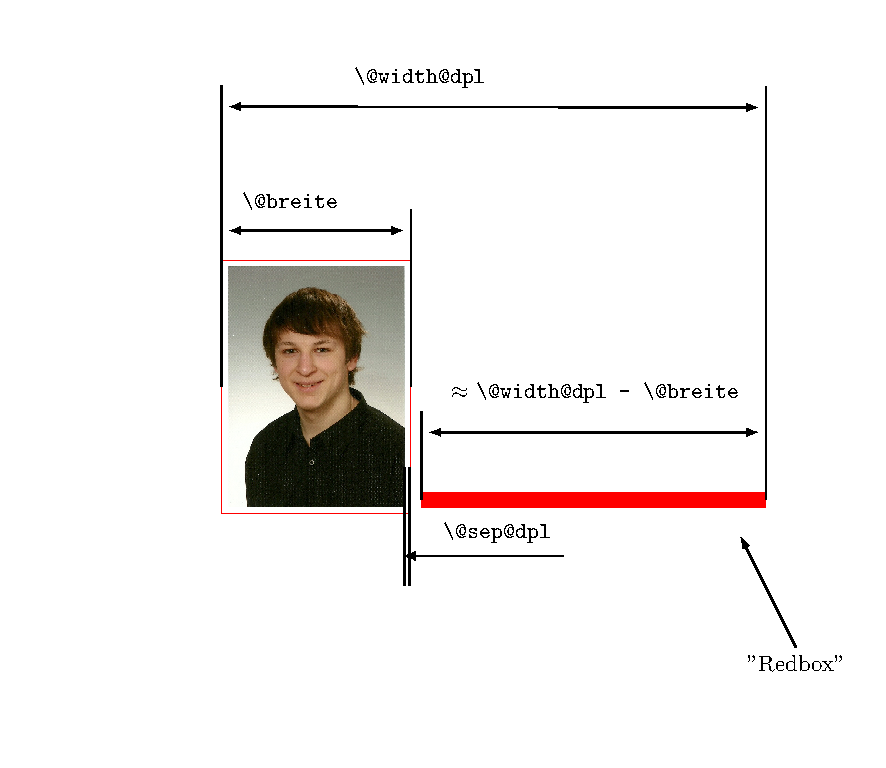
\includegraphics[width=0.8\textwidth]{Images/diplomand_erklaerung.pdf}
\caption{Festgelegte Abmessungen der Diplomandenvorstellung}
\label{pic:bemassungdipl}
\end{figure}

\textit{Anmerkung:} Abbildung~\ref{pic:bemassungdipl} beschreibt nur das Prinzip der
Ausrichtung. Es fehlt beispielsweise die Beschreibung des Abstandes zwischen \textit{Redbox} und Bild,
welcher von der Größe von \verb|\@sep@dpl| abhängt.\\ Tatsächlich
wird im Makro die \textit{Redbox} genau \verb|\@width@dpl-\@breite| breit gesetzt.
Die Gesamtbreite ist damit die eigentliche ungenaue Größe. Abbildung~\ref{pic:bemassungdipl}
ist jedoch anschaulicher als der exakte Aufbau.





%\newpage
%\phantomsection
%\addcontentsline{toc}{section}{Liste der Sourcecode Listings}
%\lstlistoflistings

\newpage
\def\refname{Literaturverzeichnis}
\phantomsection
\addcontentsline{toc}{section}{Literaturverzeichnis}

\begin{thebibliography}{abcd}
\bibitem[1]{TeXbook}{\textbf{Donald~E.~Knuth:} \emph{The \TeX{}book}. 1986, {\scshape Addison--Wesley} Verlag,\\
ISBN-13: 978-0-201-13447-6} 

\bibitem[2]{LaTeX}{\textbf{Klaus~Braune, Joachim~{\&}~Marion~Lammarsch:}\\
 \emph{\LaTeX{}--Basissystem, Layout, Formelsatz.}
2006, Springer Verlag,\\ ISBN-13: 978-3-540-00718-0}

\bibitem[3]{TikZ}{\textbf{Till~Tantau:} \TikZ{} \emph{and {\scshape pgf}--Manual for version~1.18.} 2007,\\
{\scshape gnu} Free Documentation License, Version 1.2}

\bibitem[4]{clsguide}{\textbf{The \LaTeX 3 Project:} \emph{\LaTeXe{} for class and package writers.}\\
February 2006}

\bibitem[5]{fonts}{\textbf{Carl~G.~Heise:} \emph{\LaTeX{} Kurs: Schriftarten (Kurzeinführung).}\\ TU~München, Oktober~2011}

\bibitem[6]{tugboat}{\textbf{Peter~Flynn:} \emph{Rolling your own Document Class:
Using \LaTeX{} to keep away from the Dark Side.} TUGboat, Volume 28 (2007), No. 1}

\bibitem[7]{maketitle}{\textbf{Markus~Kohm:} \emph{Titelseite mit KOMA-Script.}  Version vom 8.Juni~2011,\\
abgerufen auf \url{www.golatex.de/wiki/Titelseite_mit_KOMA-Script}}

\bibitem[8]{headings}{\textbf{Tanja~Richter:} \emph{Fußnoten, Kopf- und Fußzeilen in \LaTeX{}.} Mai~2004}

\bibitem[9]{acronym}{\textbf{Tobias~Oetiker:} \emph{An Acronym Environment for \LaTeXe .} Oktober~2010}

\bibitem[10]{websites}{\textbf{Allgemeine Foren:} \url{www.latex-community.org}, \url{www.mrunix.de},\\
									  \url{www.golatex.de}, \url{www.tex.stackexchange.com}, \url{www.texample.net}}
\end{thebibliography}\bigskip

Das Literaturverzeichnis enthält alle Quellen die zur Erzeugung und Dokumentation des Diplomarbeitstemplates
verwendet wurden. Weiters dient es zum Nachschlagen für Benutzer des Templates.\par

\end{document}